\documentclass[article]{article}

\usepackage[version = 4]{mhchem} %chem symbols and equations
\usepackage{graphicx} %graphics
\usepackage{amssymb} %math symbols
\usepackage{amsmath} %math equations
\usepackage{hyperref} %create hyperlinks: \href{link}{Word to click on}
\usepackage{amsthm}

\usepackage[sc]{mathpazo} % Use the Palatino font
\usepackage[T1]{fontenc} % Use 8-bit encoding that has 256 glyphs
\linespread{1.05} % Line spacing - Palatino needs more space between lines
\usepackage{microtype} % Slightly tweak font spacing for aesthetics
\usepackage[english]{babel} % Language hyphenation and typographical rules

\usepackage[hmarginratio=1:1,top=27mm,columnsep=20pt,left=15mm,right=15mm]{geometry} % Document margins
\usepackage[hang,small, labelfont=bf,up]{caption} % Custom captions under/above floats in tables or figures
\usepackage{enumitem} % Customized lists
\setlist[itemize]{noitemsep} % Make itemize lists more compact

\usepackage{dirtytalk} % To make cites, use \say{}

\usepackage{color}
\newcommand{\red}[1]{\textcolor{red}{#1}} 
\newcommand{\gr}[1]{{\color{red}#1}}

\usepackage{abstract} % Allows abstract customization
\renewcommand{\abstractnamefont}{\normalfont\bfseries} % Set the "Abstract" text to bold

\usepackage{titlesec} % Allows customization of titles
\titleformat{\section}[block]{\large\centering\bfseries}{\thesection.}{1em}{} % Change the look of the section titles
\titleformat{\subsection}[block]{\bfseries}{\thesubsection.}{1em}{} % Change the look of the section titles

\usepackage{fancyhdr} % Headers and footers
\pagestyle{fancy} % All pages have headers and footers
\fancyhead{} % Blank out the default header
\fancyfoot{} % Blank out the default footer
\fancyhead[C]{Physical Chemistry $\bullet$ Oct 2019 $\bullet$ Vol. XXI, No. 1} % Custom header text
\fancyfoot[RO,LE]{\thepage} % Custom footer text

\usepackage{titling} % Customizing the title section


\renewcommand{\maketitlehookd}{%
\begin{abstract}
\noindent




%% ######

\end{abstract}
}



\begin{document}
\theoremstyle{definition}
\newtheorem{definition}{Definition}[section]


\title{A computational approach to the periodic system.}

\author{%
\textsc{Andr\'es Marulanda-Bran}\thanks{Corresponding author} \\[1ex]
\normalsize Universidad de Antioquia \\ % Your institution
\normalsize \href{mailto:correoAndres}{acamilo.marulanda@udea.edu.co} % Your email address
}


\maketitle


\section{Introduction}
\label{sec:intro}

Mendeleev's periodic system is, and for the last 150 years has been, recognised as one of the most important icons of chemistry and of all of the natural sciences, both by the general public and the scientific community itself. Such a system has been shown, in several recent works, to have appeared as a natural consequence of the increasing size of the set of known substances -the chemical space-, while having as well been affected by social factors. It has been shown indeed, that the amount of chemical data was rich enough for allowing a formulation of the periodic system (PS), since as early as 1840; about 30 years before its original publication \cite{ChemSpacePSArose}.\\

The PS was devised as a means to organize and capture the generality of the chemical information of the time, which naturally consisted of chemical compositions of known substances, some of their chemical and physical properties, and some of the chemical reactions in which these were known to participate, among others. The elements were known to be interrelated to one another by two main relations: order and similarity. It is important to remark how heavily both of these concepts relied on the chemical space, for the time under study: the order relation was provided by atomic weights, which were in turn calculated by finding the lowest common weight among large sets of compounds containing a given element \cite{Hargittai:pf0063}, while similarity was assessed by comparison of the compounds elements were present in \cite{mendeleevSelectWritings}.\\

As recently reported by Leal et. al. \cite{formalStructPS}, the mathematical structure of a periodic system is, in general, that of a directed hypergraph in which elements belonging to a given hyperedge are related -say, by a similarity measure-, while order exists among \textit{and} within such hyperedges, and is not limited to one single property -e.g. atomic weight- but can arise from different orderings simultaneously. The Mendeleevian periodic table (MPT) is a special case of such a general structure, with atomic weight being the order relation used. In MPT, hyperedges are in reality partitions of the set of elements, each of these being represented by a column of the table, conforming what we call the periodic table groups. In such a setting, elements belonging to the same partition (group) are -ought to be- chemically similar, or at least more similar to the elements within the same group than to elements outside of it. \\

Taking hyperedges as mere partitions of the set of elements on a 2-dimensional array is, however, not an accurate description in general, and this was noted as early as Mendeleev's original publication of his periodic table \cite{originalMendeleev}. Paraphrasing the author: "chemically-analogous elements show either sequentially incremental atomic weights (Pt, Ir, Os), or an equal increment of this quantity (K, Rb, Cs).". Such statement can be interpreted to be referring to what, from now on, we call "horizontal" and "vertical" similarities among the MPT, respectively. \\

It is important to note that Mendeleev's approach was a purely empirical one and it depended on the known substances and elements of the time and, even further, depended on the substances a scientist knew at the time or even \textit{decided} to use for her/his analysis. \\

Mendeleev, however, didn't use the whole chemical space of his time; in fact, it has been reported that he used only very specific subsets of it, including hydrides, hydroxides, halides, oxides, and some others \cite{mendeleevSelectWritings}. In comparison, it is now known that more than 11,000 substances had been discovered by 1868, suggesting that the known chemical space was very likely undersampled, only because of its unbearable extension. In addition to this, the last 150 years have brought with them a consistently exponential increase in the size of the chemical space, with an annual growth rate of 4.4\% \cite{exponentGrowth}. For comparison, and as a consequence of this exponential growth, the number of substances reported \textit{only} in 2015, amount to the total reported between 1800 and 1950 \cite{Restrepo_2019}.\\

With a much more complete -and probably less biased- picture of 1868's chemical space, enough computational power, and inspiration from the formal formulation of the MPT, Mendeleev's original ideas of similarity shall be brought back to use on this paper. Here, we aim to extract the relationships between elements and, as a natural extension of this, the most suitable 2-dimensional representation of the PS out of such space, which may then be compared against Mendeleev's or Meyer's (or any other) periodic table. \\

All of this amounts, in principle, to questioning the fitness of \textit{a} PS, on the basis of the foundations well established 150 years ago and the available chemical space. Going even further, having obtained a way of measuring the fitness of a PS, the next step is finding an optimal configuration for this fitness measure, leading possibly to a different and more expressive PS, yet following Mendeleev's data-driven approach but in a big data setting. This approach might as well be applied yearly for the expanding set of substances, which would amount to generating a 2D representation of the periodic table for every year, which would in turn allow to explore questions such as, for instance, how stable PSs are with changes on the chemical space, and which is the first optimal date, if any, for the formulation of the PS.\\

To answer these, and other questions, this study makes use of the set of available substances discovered up to the year 2015, extracted from the Reaxys database. The article is structured as follows: Section II presents the general data-preprocessing procedure and the reasoning behind it. Section III, the calculations performed and an analysis and discussion of the results. Section IV presents an optimization setting for the PS with (probably, but not quite yet) possible candidate configurations and the analysis of these results.\\


\section{Data description and preprocessing}
\label{sec:preprocessing}

The compositional formulas of all the available compounds were extracted from the database in such a way that the resulting data is a collection of text strings such as for instance C6H12O. It is worthwhile noting that this approximation ignores every structural factor and relies only on compositional data, which in turn disregards any information about isomers.\\

The main goal at this point is to convert this corpus of strings into a data representation that directly expresses relationships between elements. For such a task, the underlying "grammar" behind each compound's composition is to be found, and for that matter the processing and analysis must be focused on interactions between compounds rather than the conversion of single compounds into machine-readable formats. Note that this approach differs from usual machine learning studies in that in these, the latter formats are constructed and given to an algorithm, with the structure of the data being looked for $\textit{after}$ training; while the  approach presented here aims to directly extract structure from the data, allowing to make analyses and conclusions before any statistical learning is invoked.\\

Very much in the spirit of Mendeleev's concept of similarity: \say{The elements, which are most chemically analogous, are characterized by the fact of their giving compounds of similar form RXn}, our preprocessing consists of decomposing all the available compositional formulas, into all possible rewritings of the form $R-X_n$. In this rewriting, X is any single element and n is a subindex, while R can be any combination of elements with subindices, possibly including element X too. As an example, the compound $\ce{SiCl4}$ can be rewritten as $\ce{SiCl3-Cl}$, $\ce{SiCl2-Cl2}$, $\ce{SiCl-Cl3}$, $\ce{Si-Cl4}$, and $\ce{Cl4-Si}$. Note that, at this point, chemical compositions of substances of various sizes and elemental compositions have been converted into a "binary compound" representation, which allows already for an important increase in the size of the dataset, with which studies such as \cite{Leal2012}, where only binary compounds (nearly 4700) were used for a network study, may be reworked to yield important results with a naturaly much less biased picture of the chemical space. \\

For our purposes here, we regard a similarity relationship between two elements, as follows:

\begin{definition}[Similarity relationship]
\label{def:def1}
Two elements X and Y are connected through a similarity relationship (R,n), iff there exist two compounds $A = R-X_n$ and $B = R-Y_n$, such that substitution of n atoms of X in compound A, by n atoms of Y, would result in compound B.
\end{definition}

In practice, sets of elements were constructed to represent such similarity relationships and, as such, a set of elements is constructed for each pair (R,n). An example of the computation is as follows: assuming the compounds $\ce{KOH}$, $\ce{NaOH}$ and $\ce{H2O}$ exist, then by this treatment a set {K, Na, H} will be formed corresponding to the similarity relationship (OH,1). Naturally, all sets of cardinality equal to one were removed as they contain no information about relationships between elements.\\

Note that this approach assumes that $n \in \mathbb{N}$, that is, a problem arises when considering non-stoichiometric compounds. In the given dataset examples of such non-stoichiometric compounds were found, and so this case needs to be properly handled. Although it was observed that some of these compounds correspond to crystalline phases with non-stoichiometric amounts of water molecules, implying that the dataset could be manually curated in order to include such substances, it was decided to ignore them for the sake of simplicity. \\

\subsection{Results of preprocessing}
Starting from more than 19 million compounds obtained after removing non-stoichiometric entries, further data reduction was obtained from the removal of isomers. As we are interested in historical analyses, and various isomers are discovered in different years, the effective year for each compositional formula was decided to be that of the earliest discovered isomer, which corresponds to the date of report of said composition formula. After such cleaning, nearly 3.5 million different formulas were obtained, upon which the previously discussed preprocessing procedure was applied.\\

A total of more than 280 million unique \say{binary compound representations} (rewrittings of the form RX$_n$) were obtained, from which more than 9.5 million different similarity relationships were extracted. Note that these \say{similarity relationships} relate, in general, more than two elements, so the actual number of binary similarity relationships within our dataset is much larger than this number. The actual number of such binary relations can be calculated as the sum of the number of 2-combinations of N$_i$, the cardinality of set i. Such quantity is equal then to $\sum_i \binom{N_i}{2}$.\\

\section{Results and discussion}

\subsection{Similarity matrices}

As explained above, a sense of similarity between a pair of elements is extracted from the number of similarity relationships joining them. This similarity between pairs of elements is what can then be used as one of the dimensions of a PS and is thus of central importance to the present analysis.
For that reason the concept of similarity matrix is formulated as follows.

\begin{definition}[Count matrix]
\label{def:CountMatrix} 

Let L be a sorted list of the elements, and N be the length of such list.
The elements $M_{ij}$ of a Count Matrix are defined as the number of similarity relations found between elements i$^{th}$ and j$^{th}$ of list L. In the case i=j, $M_{ii}$ is defined as the number of similarity relations i$^{th}$ element is found in.

\end{definition}

\begin{definition}[Similarity matrix]
\label{def:simMat} 

Let L be a sorted list of the elements, and N be the length of such list.
Then a similarity matrix S is an NxN matrix, where entry $S_{ij}$ represents a net similarity measure between the i$^{th}$ and j$^{th}$ elements of list L. 
Such matrix is defined on the basis of Count Matrix M as follows:

	\begin{equation}
		S_{ij} = \sqrt{\frac{M_{ij}^2}{(\sum_{i'}{M_{i'j}})(\sum_{j'}{M_{ij'}})}}
	\end{equation}

\end{definition}

With this definition at hand, similarity matrices were calculated for each year between 1800 and 2015. As will be explored in detail later on, these matrices show patterns that can be correlated with and understood under the light of the well known MPT.\\


\subsubsection{Similarities: 1868}
Let us now explore the similarities between elements for the year 1868. The numbers shown here represent a result of the analysis discussed earlier, performed over a dataset limited to the substances discovered before this year only; as such, only 60 elements are present in the matrix. This year is of primal relevance for this study, as this is the year of first publication of Mendeleev's PS and, as such, studying relations between elements for this particular moment of history allows for the exploration of the relations upon which Mendeleev and others based the construction of their periodic systems.\\

Figure \ref{fig:simMat1867} shows the similarity matrix, as defined in def. \ref{def:simMat}, calculated with the compounds known before the year 1868. In this plot, a darker color implies larger similarity between a pair of elements. Additionally, for purposes of visualization, all diagonal elements were set to 0 as it is understood these are by definition the largest entries on the matrix (equal to 1).\\

\begin{figure}[h!]
  \centering
	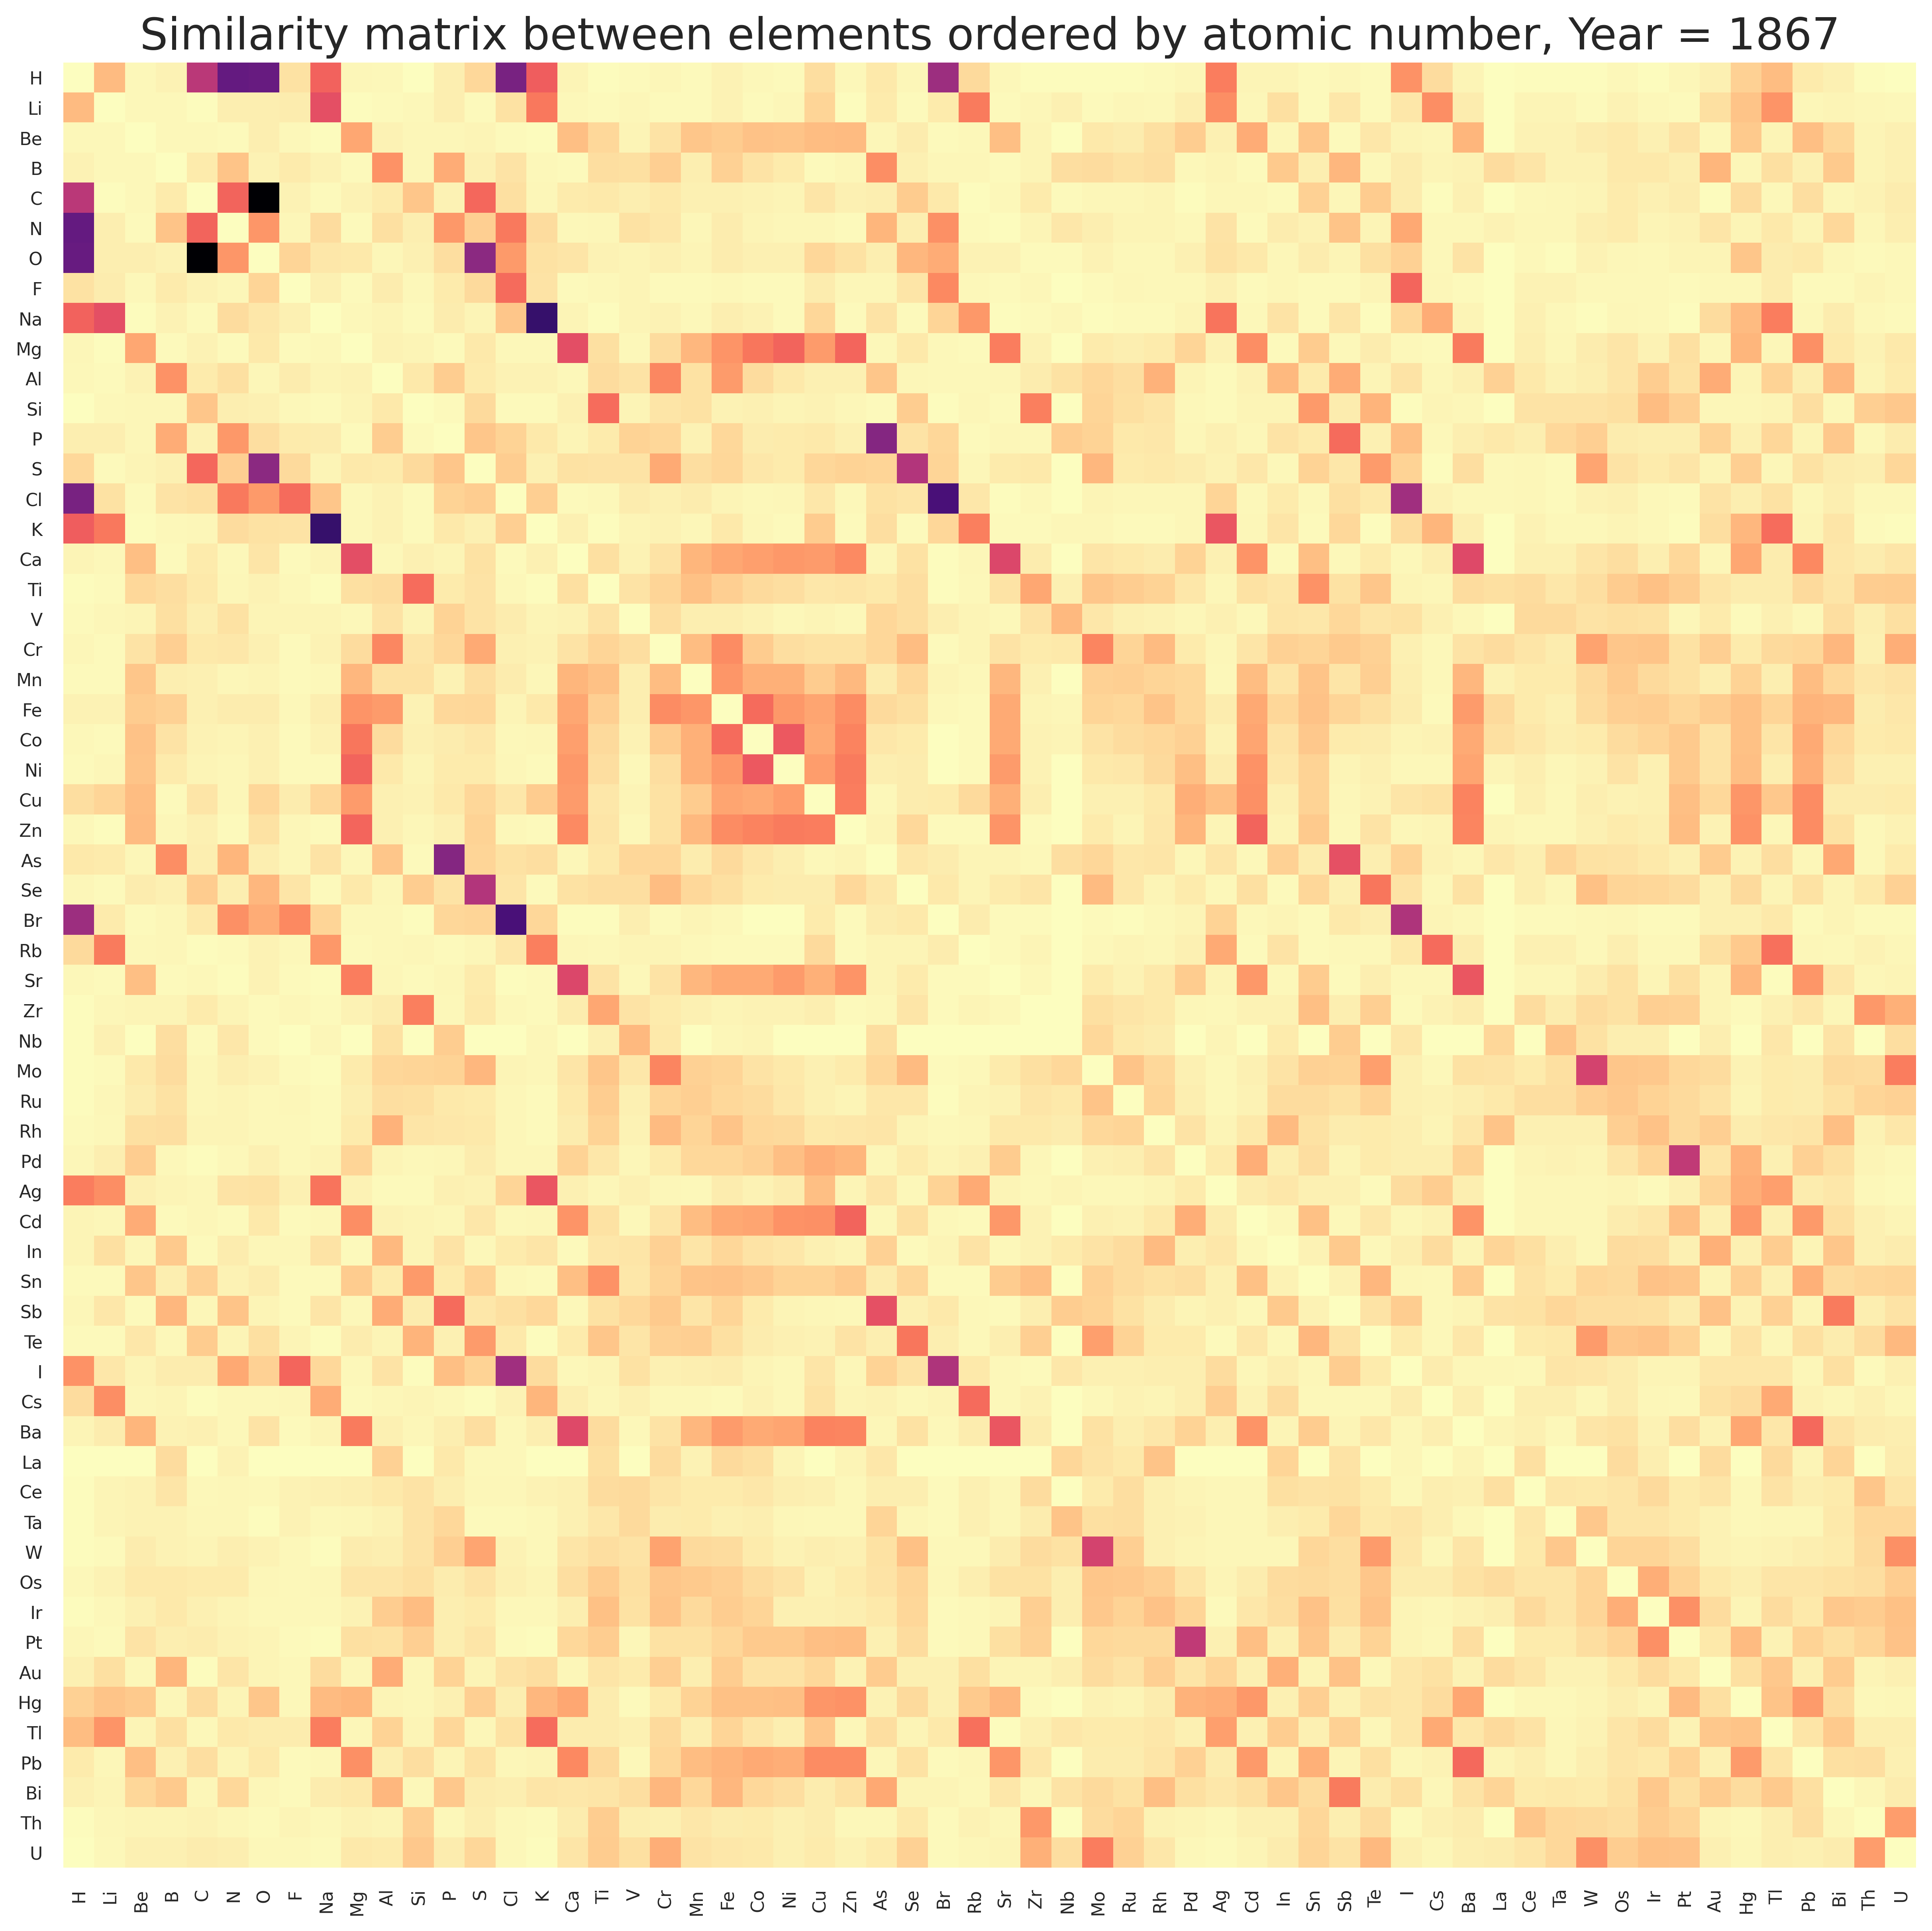
\includegraphics[width=10.0cm]{simMat1867.png}
	\caption{Similarity matrix for year 1868.}
	\label{fig:simMat1867}
\end{figure}

In general terms and as anticipated, some substructures can be seen within the matrix such as, for instance, vertical, horizontal and more prominently diagonal lines, which explicitly suggest the higher structure the PS is intended to capture. These diagonals, as will shortly be explained, are reminiscents of what will then be realised in the MPS as vertical, or group similarities. \\

To understand the meaning of these diagonals, let us explore one of the most prominent of these in figure \ref{fig:simMat1867}; the diagonal starting from the relation As $\rightarrow$ P, followed by Se $\rightarrow$ S, and so on. Both of these are realised as sequential, pair-wise vertical similarities in MPT. In general terms, provided entry $M_{jk}$ has a high value, the fact that entries $M_{j+n,k+n}$, n integer, are high as well, is reminiscent of the periodic behaviour expressed in the construction of groups in MPT. As can be seen, such diagonal patters are repeated all over the matrix implying a higher order pattern, which would allow for the formation of whole groups of elements, as is done in MPT.\\

Other patterns are prominent too, such as vertical lines that are repeated in the horizontal direction, forming what can be understood as another periodic pattern. These are realised as horizontal and non-local relationships in MPT, meaning by non-local that such similarities are not encoded as closeness in MPT. In particular, a bright block is formed by the elements from Cr to Zn, which represents the well known horizontal similarity among first row transition metals. In addition, the repeating vertical lines to the sides of this block correspond each to one of the elements of group 2 of MPT, plus Hg and Pb. Such relation between first row transition elements and group 2 elements is by no means encoded in MPT, indicating a lack of dimensionality of this tabular representation.\\

One particularly important element for our discussion is hydrogen, as its position in the PT is still a controversial matter [cite]. Arguments from electronic structure arise for the placement of H on the first group, as its valence shell contains one electron [cite], or on the 17th group (the halogens), as it lacks one electron for a full valence shell [cite]. There are even arguments stating that H should be on 14th group, above Carbon, as its valence shell is half full [cite]. In Figure \ref{fig:repH}, a plot is provided based on the current approach, that is intended to contribute to the discussion. 

\begin{figure}[h!]
  \centering
	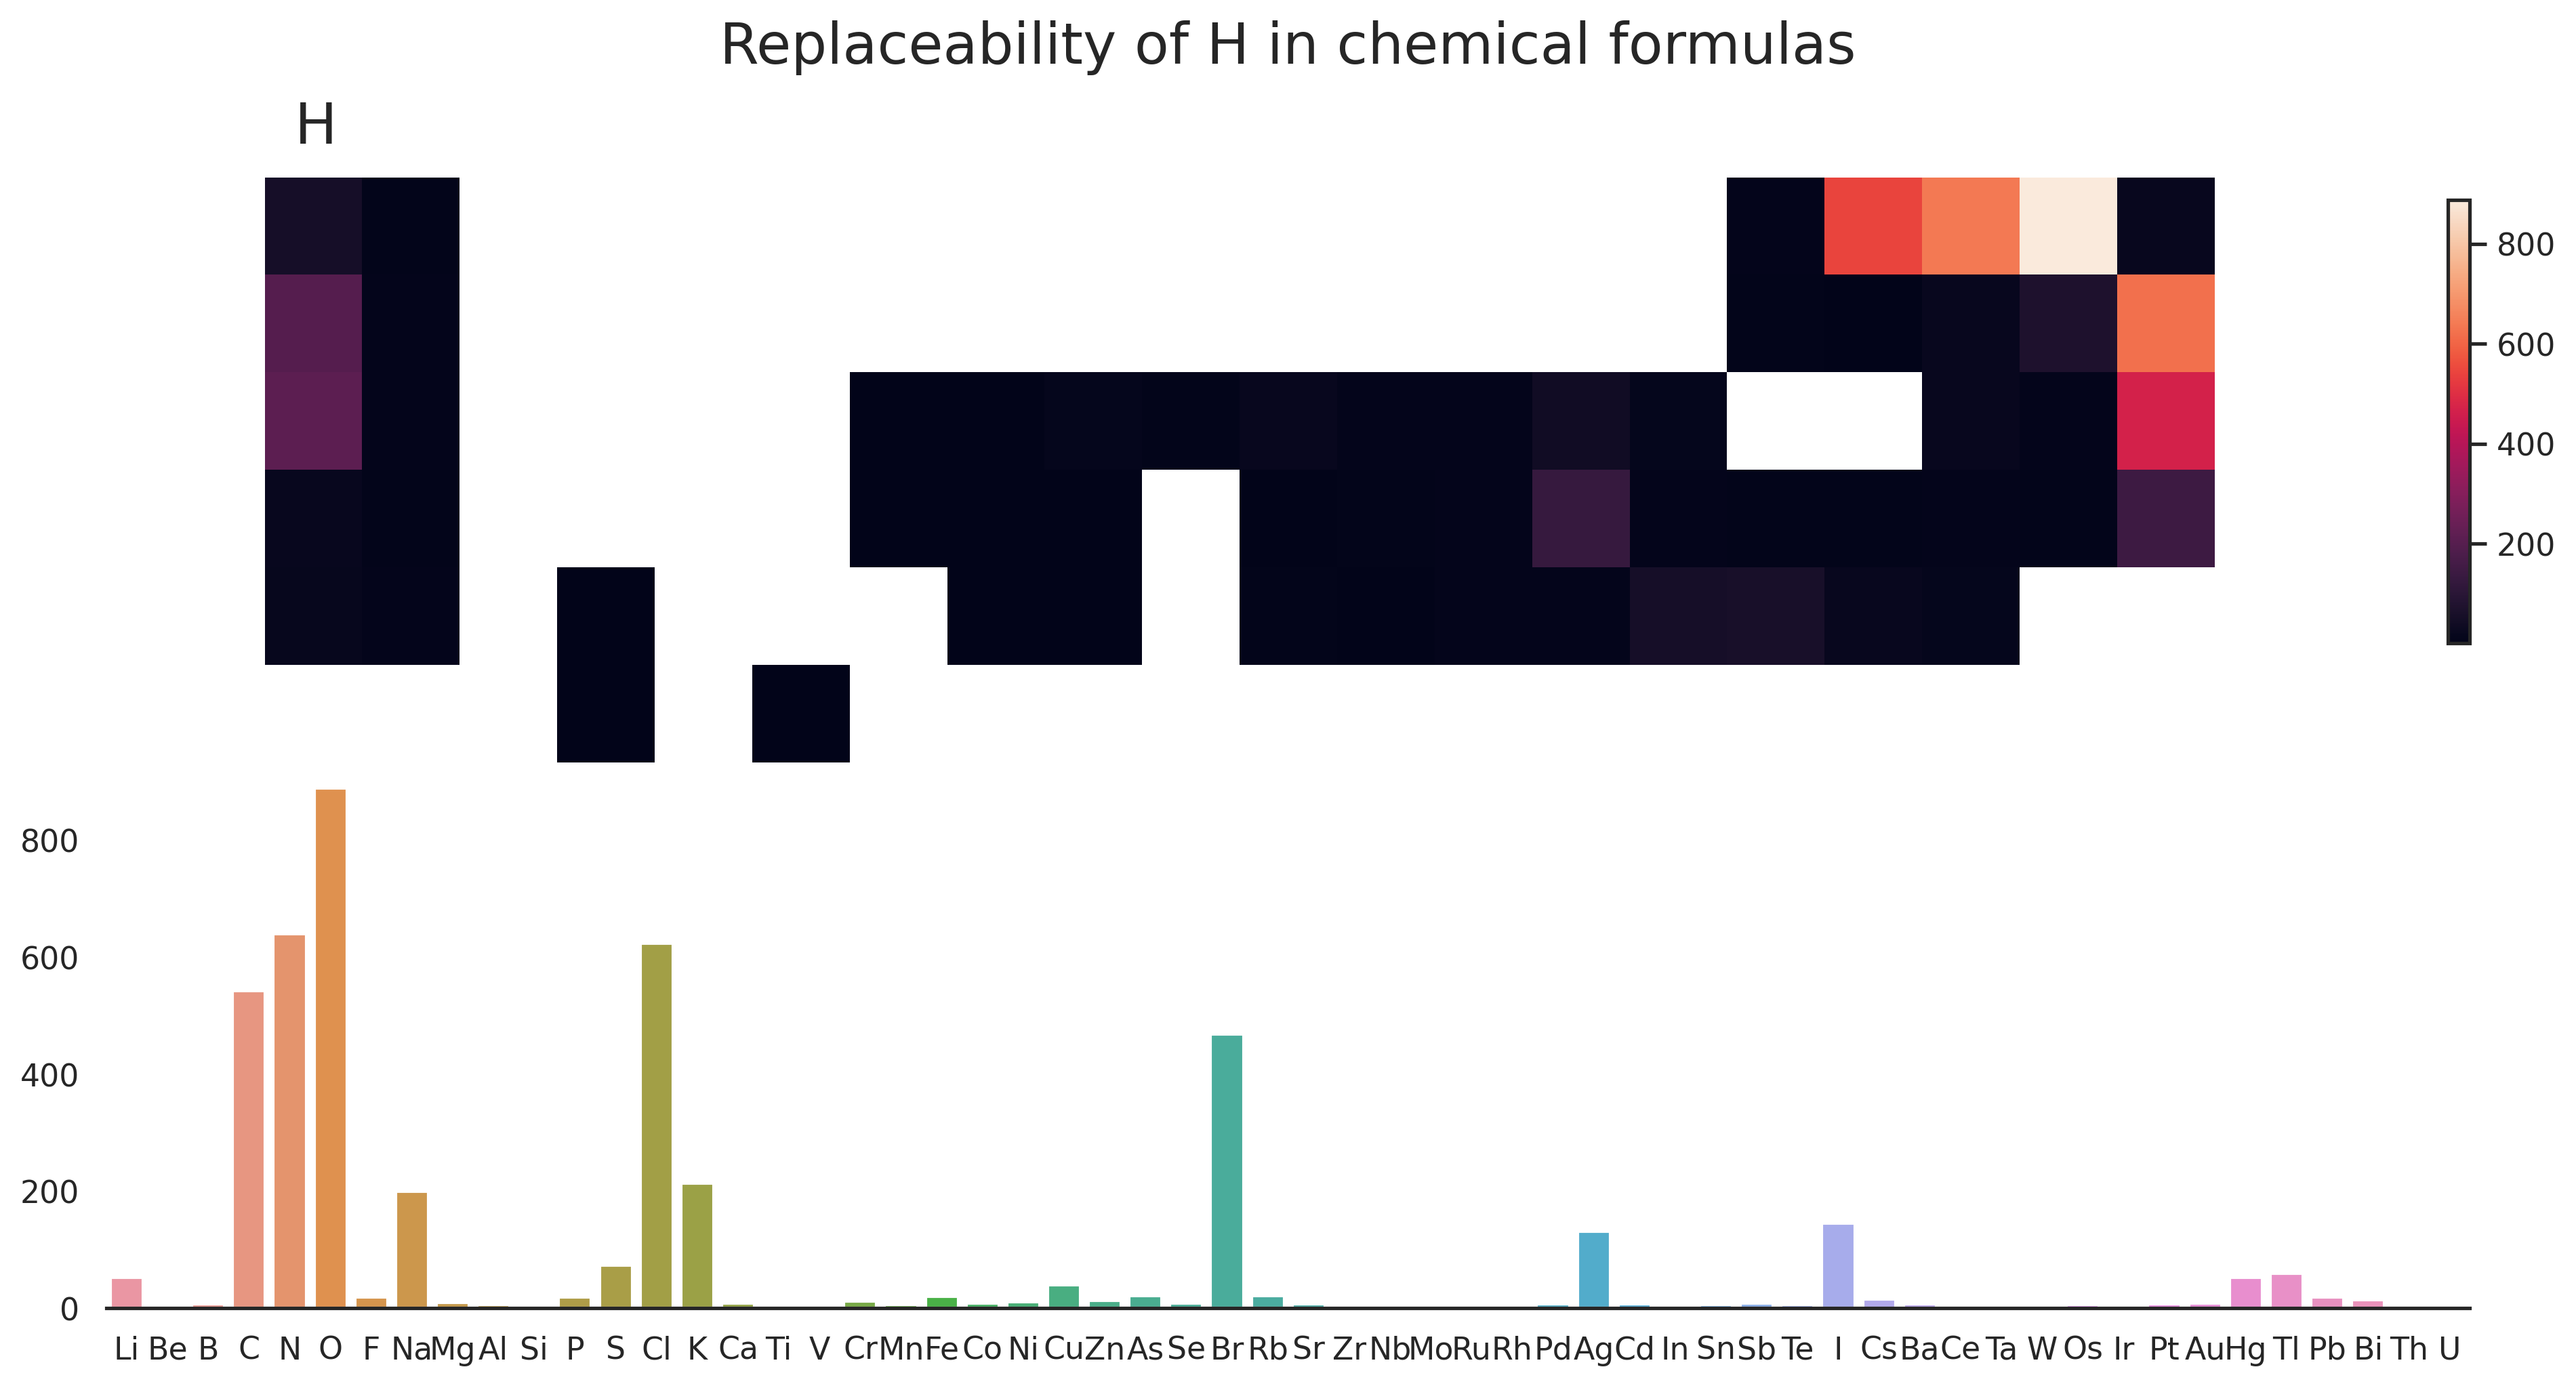
\includegraphics[width=13.0cm]{replace_H.png}
	\caption{Replaceability of H in compounds in dataset. Year 1868.}
	\label{fig:repH}
\end{figure}

The results shown in Figure \ref{fig:repH} show that H can be frequently replaced, expectedly, by Na and K, one of the groups it is attached to. Evidence is also provided, that H is even more similar to the halogens, as replaceability of H is higher for Cl, Br and I to a lesser extent. More prominently, however, strong relationships with O, C, and N are observed, which contribute to a much more interesting discussion: that of whether H should be a group 14 element.\\

The latter relations may seem exotic at first, however, the composition formulas responsible for this result offer an explanation. Substances such as $\ce{SX2}$, $\ce{OTlX}$, $\ce{NX3}$, $\ce{MoOX}$, $\ce{MnOX}$ and others alike are found for the case of the relation H $\rightarrow$ O. These show that such a result is actually due to the presence of metallic oxides, hydroxides and hydrides, and happens in combination with elements with more than one oxidation state such as transition metals and other non-metals such as S and N, which allows them to combine in some compounds with a number $\textit{x}$ of Hs, while in other compounds with the same number of Os by doubling their oxidation state.\\

With the aim of exploring how these trends evolve with time, let us now explore the similarity matrix calculated for the year 2015, which corresponds to the most complete picture available to this point.

\subsubsection{Similarities: 2015}

Figure \ref{fig:simMat2015} shows the results of the same calculation, as explained in the previous section, but with the whole dataset. This corresponds to the most complete map of similarities between elements that can be achieved with the current treatment and, as such, represents one of the most important products of this research. \\

\begin{figure}[h!]
  \centering
	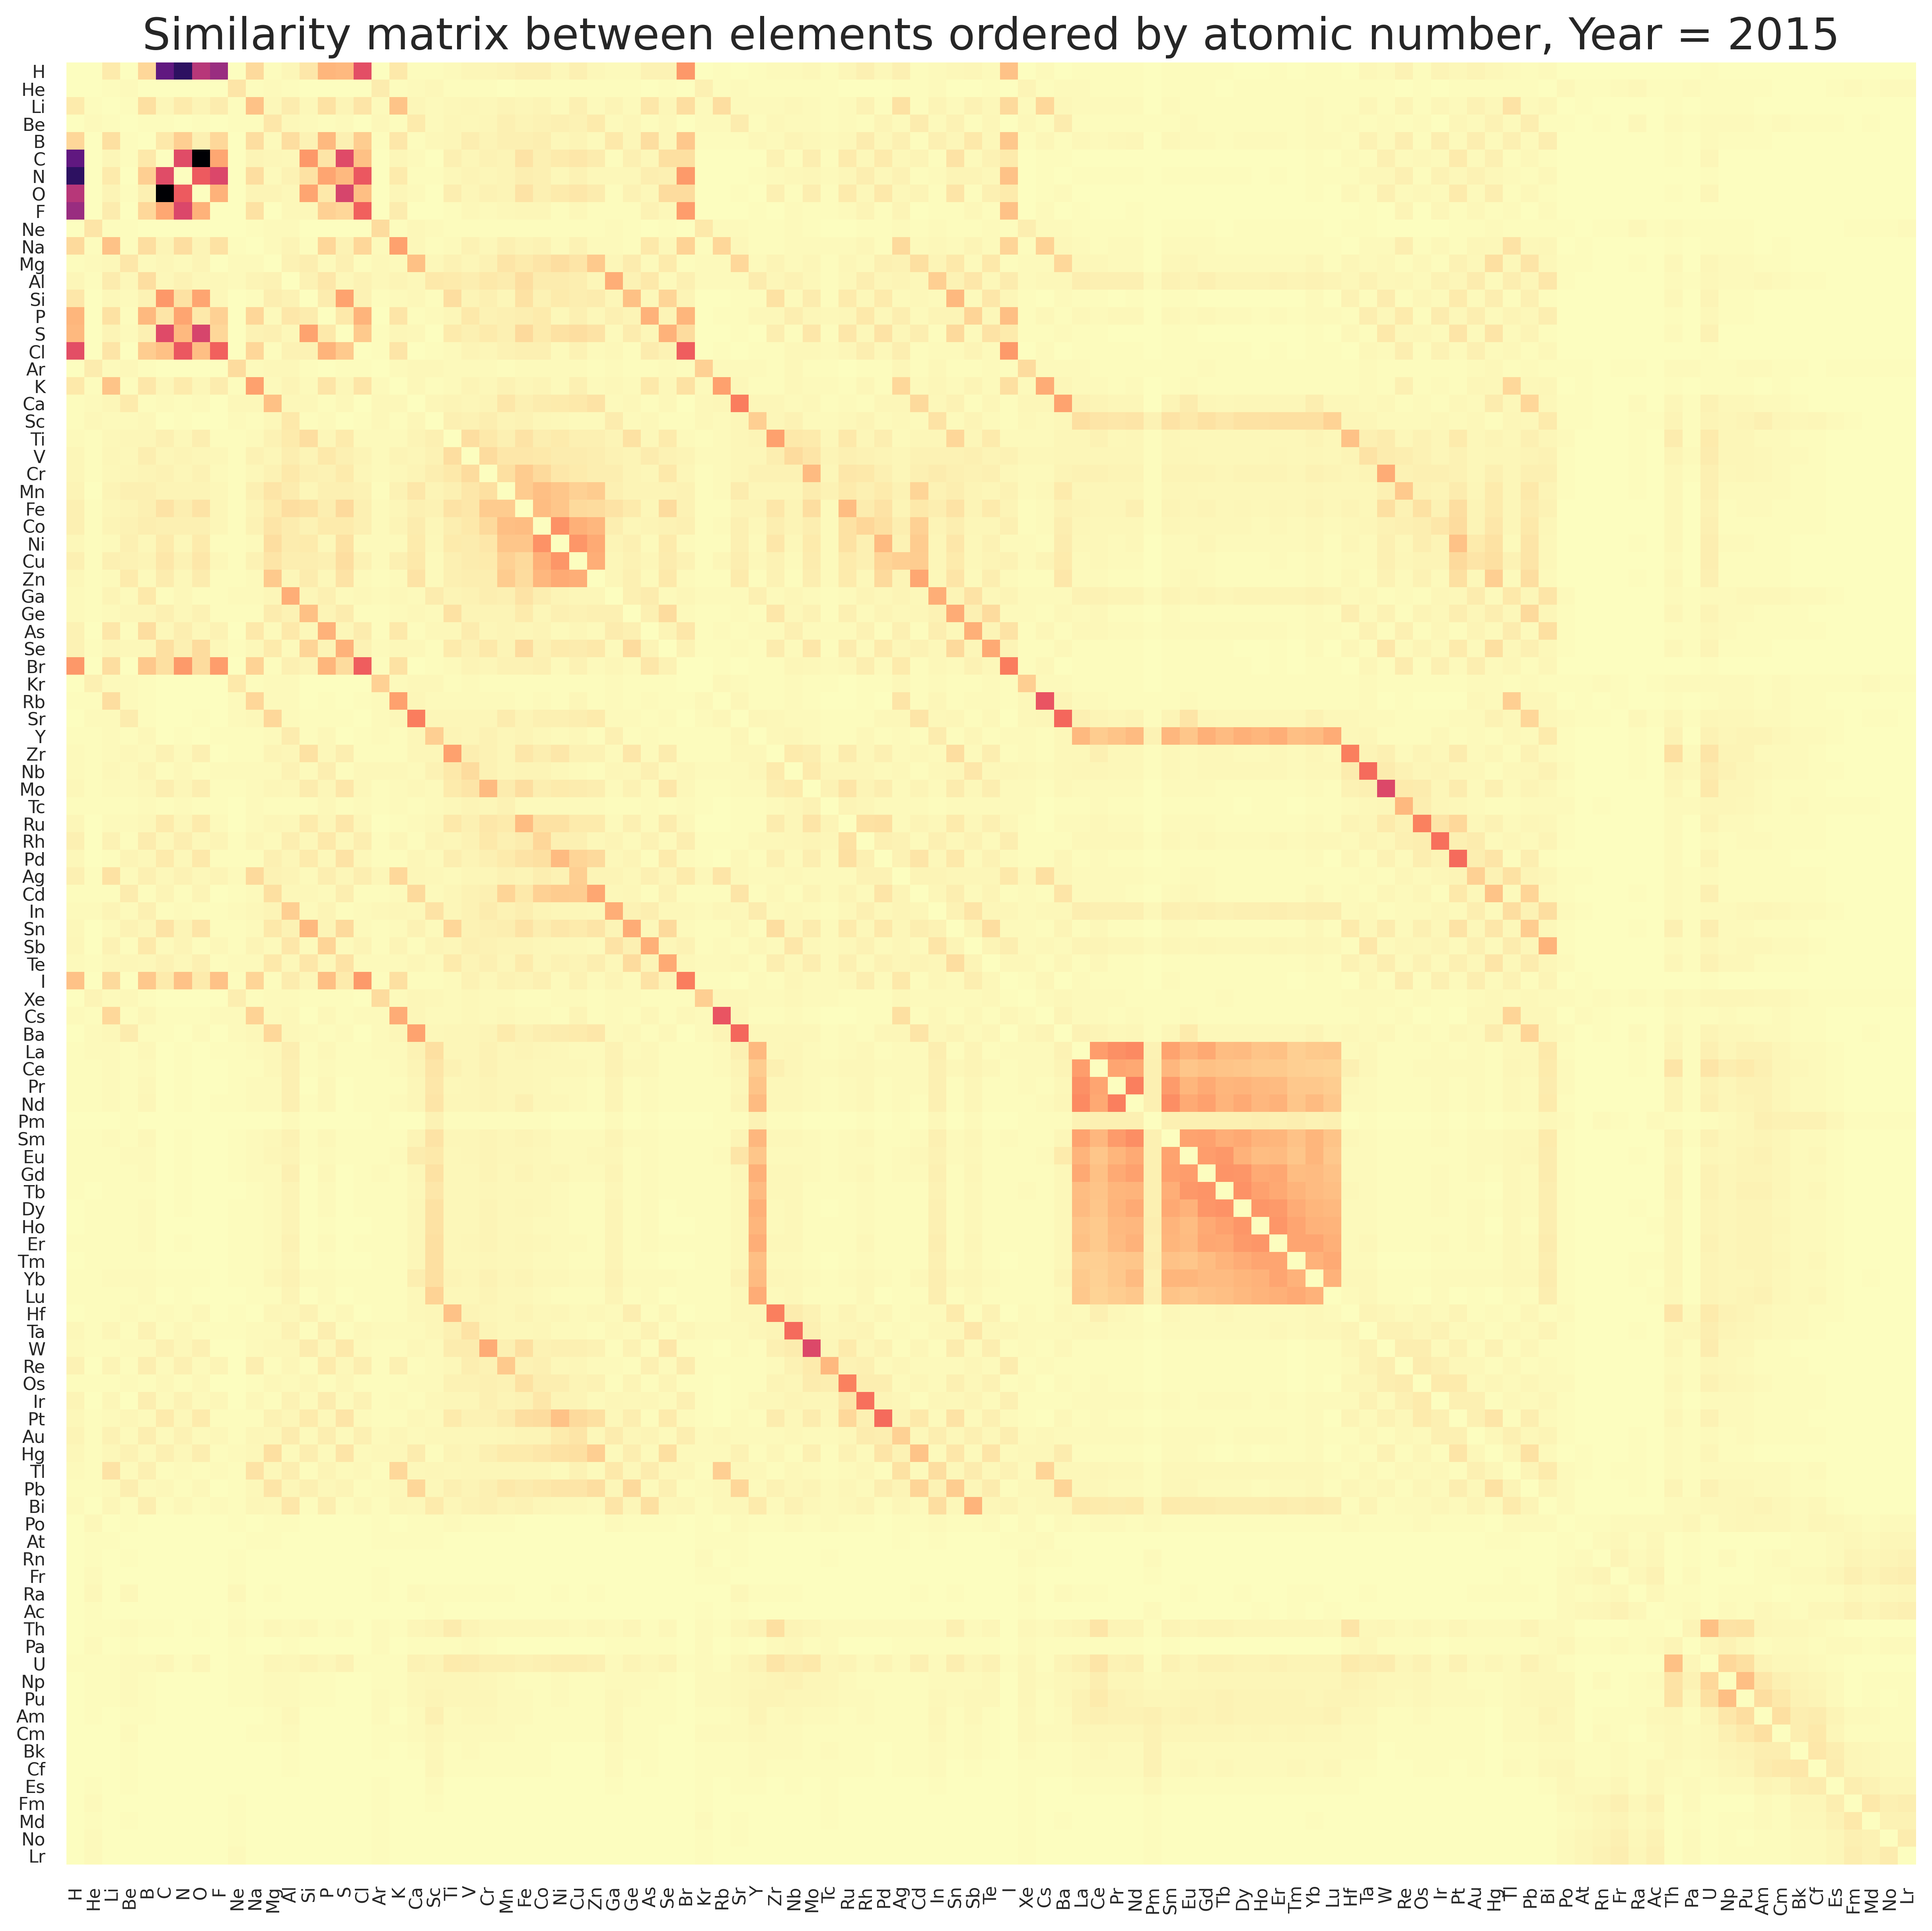
\includegraphics[width=12.0cm]{simMat2015.png}
	\caption{Similarity matrix for year 2015.}
	\label{fig:simMat2015}
\end{figure}

In the light of the analyses earlier discussed, the results in figure \ref{fig:simMat2015} are quite interesting, as they seem to imply that the periodicity and the other relationships above discussed, are preserved and even \textit{reinforced} with time, even with the introduction of more than 40 new elements since 1868.\\

A whole new group of elements is introduced to the study, namely, the lanthanides. These show remarkably high and consistent similarities within the series, being the responsible for the bright large square in the middle of the matrix. Other manifestations of periodicity are observed too, this time more prominently than in the previous plot. Here, the diagonals go ver clearly and uninterruptedly, from Zn $\rightarrow$ Mg, all the way to La $\rightarrow$ Y, where a vertical relation is shown (i.e. Y $\rightarrow$ La - Lu), and then the diagonal pattern is continued, starting from Hf $\rightarrow$ Zr and, arguably, going as far as down to Bi $\rightarrow$ Sb.\\

There are other less clear, but similar patterns. It is observed, for instance, an additional diagonal formed starting from Ag $\rightarrow$ Na, all the way down to Ba $\rightarrow$ Ca, where it is interrupted by a  vertical pattern correspondent to similarities between Sc and the lanthanides (La-Lu). The diagonal pattern is again observed starting from Hf $\rightarrow$ Ti, down to Bi $\rightarrow$ As. Such diagonal-vertical-diagonal pattern is found to be repeated with some periodicity at least 4 times in the whole matrix, and decreases in intensity with the distance from the main diagonal on the matrix ($S_{ii}$). \\

Many things can be said just from these results. The lanthanides are observed to be a highly consistent group, meaning that all the elements here are very similar to all other elements in the same group. Additionally, the results in figure \ref{fig:simMat2015} and the discussion above provide evidence that Y and, to a lesser extent, Sc, behave much like lanthanides, a fact discussed in earlier works [cite]. The less intense patterns discussed in the last paragraph, express a vertical, non-local similarity between elements in MPT, such as that expressed by Ga $\rightarrow$ Ti. Similar connections are observed since Ag $\rightarrow$ Na and, less prominently, Mg $\rightarrow$ Cd, indicating the possibility that Na and Mg be placed above Cu and Zn, respectively. Such relations were noted by Mendeleev as early as his 1871 publication of the PS, to the extent that Ag was grouped with the alkaline elements and Cd with the alkaline-earths.\\

Many questions arise on the light of these results. Importantly, the focus of this work is on PSs and their evolution, and as such the interest relies on automatic extraction of such systems, and the analysis of their time evolution. This will be the topic for the following sections.

\in 

\subsection{Automatic generation of periodic system representations}
\label{sec:geneticAlgo}

On the previous section it was shown how similarity matrices, framed within the methodology for assessment of similarities introduced by the present work, do indeed uncover patterns that can be correlated with the observations of, for instance, the MPT. The question that arises is, however, whether it is possible to automatically extract a periodic system representation (PTR) out of such results. This is important for a number of reasons, but more importantly, it would allow a direct \say{mapping} from CS to PTR, which could then be applied to the evolving CS to address the question about the historical evolution of the PS. On the other hand, the \textit{stability} of the PS may be investigated in a similar way, in that case by introducing perturbations to the CS and evaluating the variation on the resulting PS.

This section introduces an approach to such automatic generation of PSs, and explores various approaches for different types of representations. \\

A PTR can have possibly many shapes, dimensions, and have various other different mathematical properties. As originally proposed by Pettifor [cite Pettifor], one such representation can be built in one dimension, on the base of information about similarity. In particular, the PTR would consist of an optimal ordering, or ranking of elements, such that similar elements are placed together or in nearby positions. The work in \cite{Glawe_2016} was a reformulation of the original Pettifor's scale, using a similar approach to the one presented here, but using only a set of inorganic substances obtained from \href{https://ucsd.libguides.com/crystallography/icsd}{the ICSD}. Again, such work could highly benefit from the more general approach considered here with much more substances and a deeper extraction of relations, and the conclusions of such work could as easily be drawn from this treatment.\\

With such a task in mind, a genetic algorithm was implemented, as done in \cite{Glawe_2016}. The crossover and mutation operators used were the same as indicated in the reference. The only difference from their approach is that in the implementation used for this work, the endpoints are not fixed and can be any element, while in their work the endpoints were fixed to be H and Kr. The optimization objective (loss function) used was the same as that used by the reference (eq. \ref{eq:eq2}), as it takes into account the distances between all pairs of elements in the given ordering $i$, and weights each contribution with the elements $S_{AB}$ of a similarity matrix. It penalizes similar elements being far from each other in the sequence, regardless of their particular position within it.

\begin{equation}
	\label{eq:eq2}
	F = -\sum_{A,B \neq A} \frac{S_{AB}}{|i_A - i_B|}
\end{equation}

Having set up both an optimization algorithm and an objective function, some benchmarks were calculated before any optimization was tried. In particular, the cost associated with the following orderings were calculated, using eq. \ref{eq:eq2} and the similarity matrix calculated for the CS of 2015: Random Orderings, Atomic Number (AN), Pettifor's original scale (POS), Glawe's genetic algorithm  scale (GGA). For the random orderings, the loss usually lies between -4 and -5, while for AN it's -8.66, for POS is -12.56 and finally for GGA is -12.63. 

This shows in fact that the similarity matrix calculated here captures in escence the same patterns as that calculated in \cite{Glawe_2016}, as the patterns in losses for different scales are preserved.\\

With such benchmarks at hand, 20 optimizations were carried on in parallel and the best \textit{individual} out of each experiment was selected as a representative of the \textit{population}. Such an amount of experiments were performed to account for the variability on the results, as the optimization method used is inherently random. The obtained losses lie between -13.31 (maximum) and -14.09 (minimum). Compared to the reference, these results are considerably better as they improve the loss function in more than 1 point with respect to POS, while the improvement of Glawe's results with respect to the same reference are less than 0.1 with our dataset. \\

As expected, given the randomness of the method, the 20 orderings obtained through optimization for 2015 were in many cases not directly comparable. Such orderings, however, shared common features in the way elements were ordered; in particular, some PT groups can be recognised in most of the optimized PTRs. Furthermore, and as explained before, the calculated costs for such orderings represent an improvement with respect to the baselines in all 20 cases. \\

A metric was devised that allows for the comparison of different orderings in terms of the conservation of \textit{local features} from one ordering to the other. Such a metric is important to this work as it allows for two things in principle: 1. The comparison of orderings optimized under the same CS, giving a measure of variability of a PS for a given year; and 2. The direct comparison between the PTRs optimized under the CS of two different years, which in turn would allow a large scale historical analysis that can be used to address questions about the stability or, if any, convergence of the PS with time. \\

\subsection{Comparison of 1D PTRs}

\equiv
\subsection{Historical evolution of the PS}

Equiped with time-evolving CSs, and methods for obtaining PTRs out of such CSs and comparing them, a historical analysis is now straightforward, in the sense that all there is to do now is generating PTRs for each year to consider in the analysis, and comparing the results as a function of time.\\

For this section, 20 optimization procedures were carried out in parallel for each even year, between 1800 and 2016. The best individual out of such procedures was selected, so that for each year 20 ---possibly different--- orderings were obtained. Next, the PTRs of one year $Y_1$ against those of another year $Y_2$ are compared. As there are 20 orderings for each year, the quantity reported here when comparing $Y_1$ with $Y_2$ is the average similarity of all 400 possible resulting combinations of orderings from one year to those of the other. \\

Notice that the number of known elements increases with time, and that it is considerably low during the first century, as compared to more recent years. Such evolution is shown in figure \ref{fig:numElems_evol}. It would then be unfair to directly compare a PTR from 1820 with one from 1980 as nothing can be said in 1820 about the relative orderings of, e.g. the lanthanides. With this in mind, the only correction that needs to be made to our similarity measure is changing the normalization factor. In our implementation, the normalization factor was calculated in an asymmetric manner, so that a single value resulting from the comparison of $Y_1$ against $Y_2$ is normalized using the normalization factors derived from the lengths of each of the orderings. The results of such an analysis are presented in figure \ref{fig:historicAnal}. \\

As explained, the similarities are normalized by the year displayed on the vertical axis. A conceptual distinction must be made between the values above and below the diagonal. In particular, values below the diagonal correspond to a comparison from the point of view of the earliest year, which helps address the question: Up to what extent do relationships found in year $Y_1$ (past) are preserved in the future years?. Meanwhile, above the diagonal the opposite is found. In this region we find a comparison from the privileged point of view of the future observer, against previous years. The question here would then be: What proportion of the relationships found in year $Y_2$ were already known years before? This part of the plot naturally contains lower values, a fact mainly driven by the lack of information about newer elements that existed in previous years, as compared to more recent years.\\

\begin{figure}[h!]
  \centering
	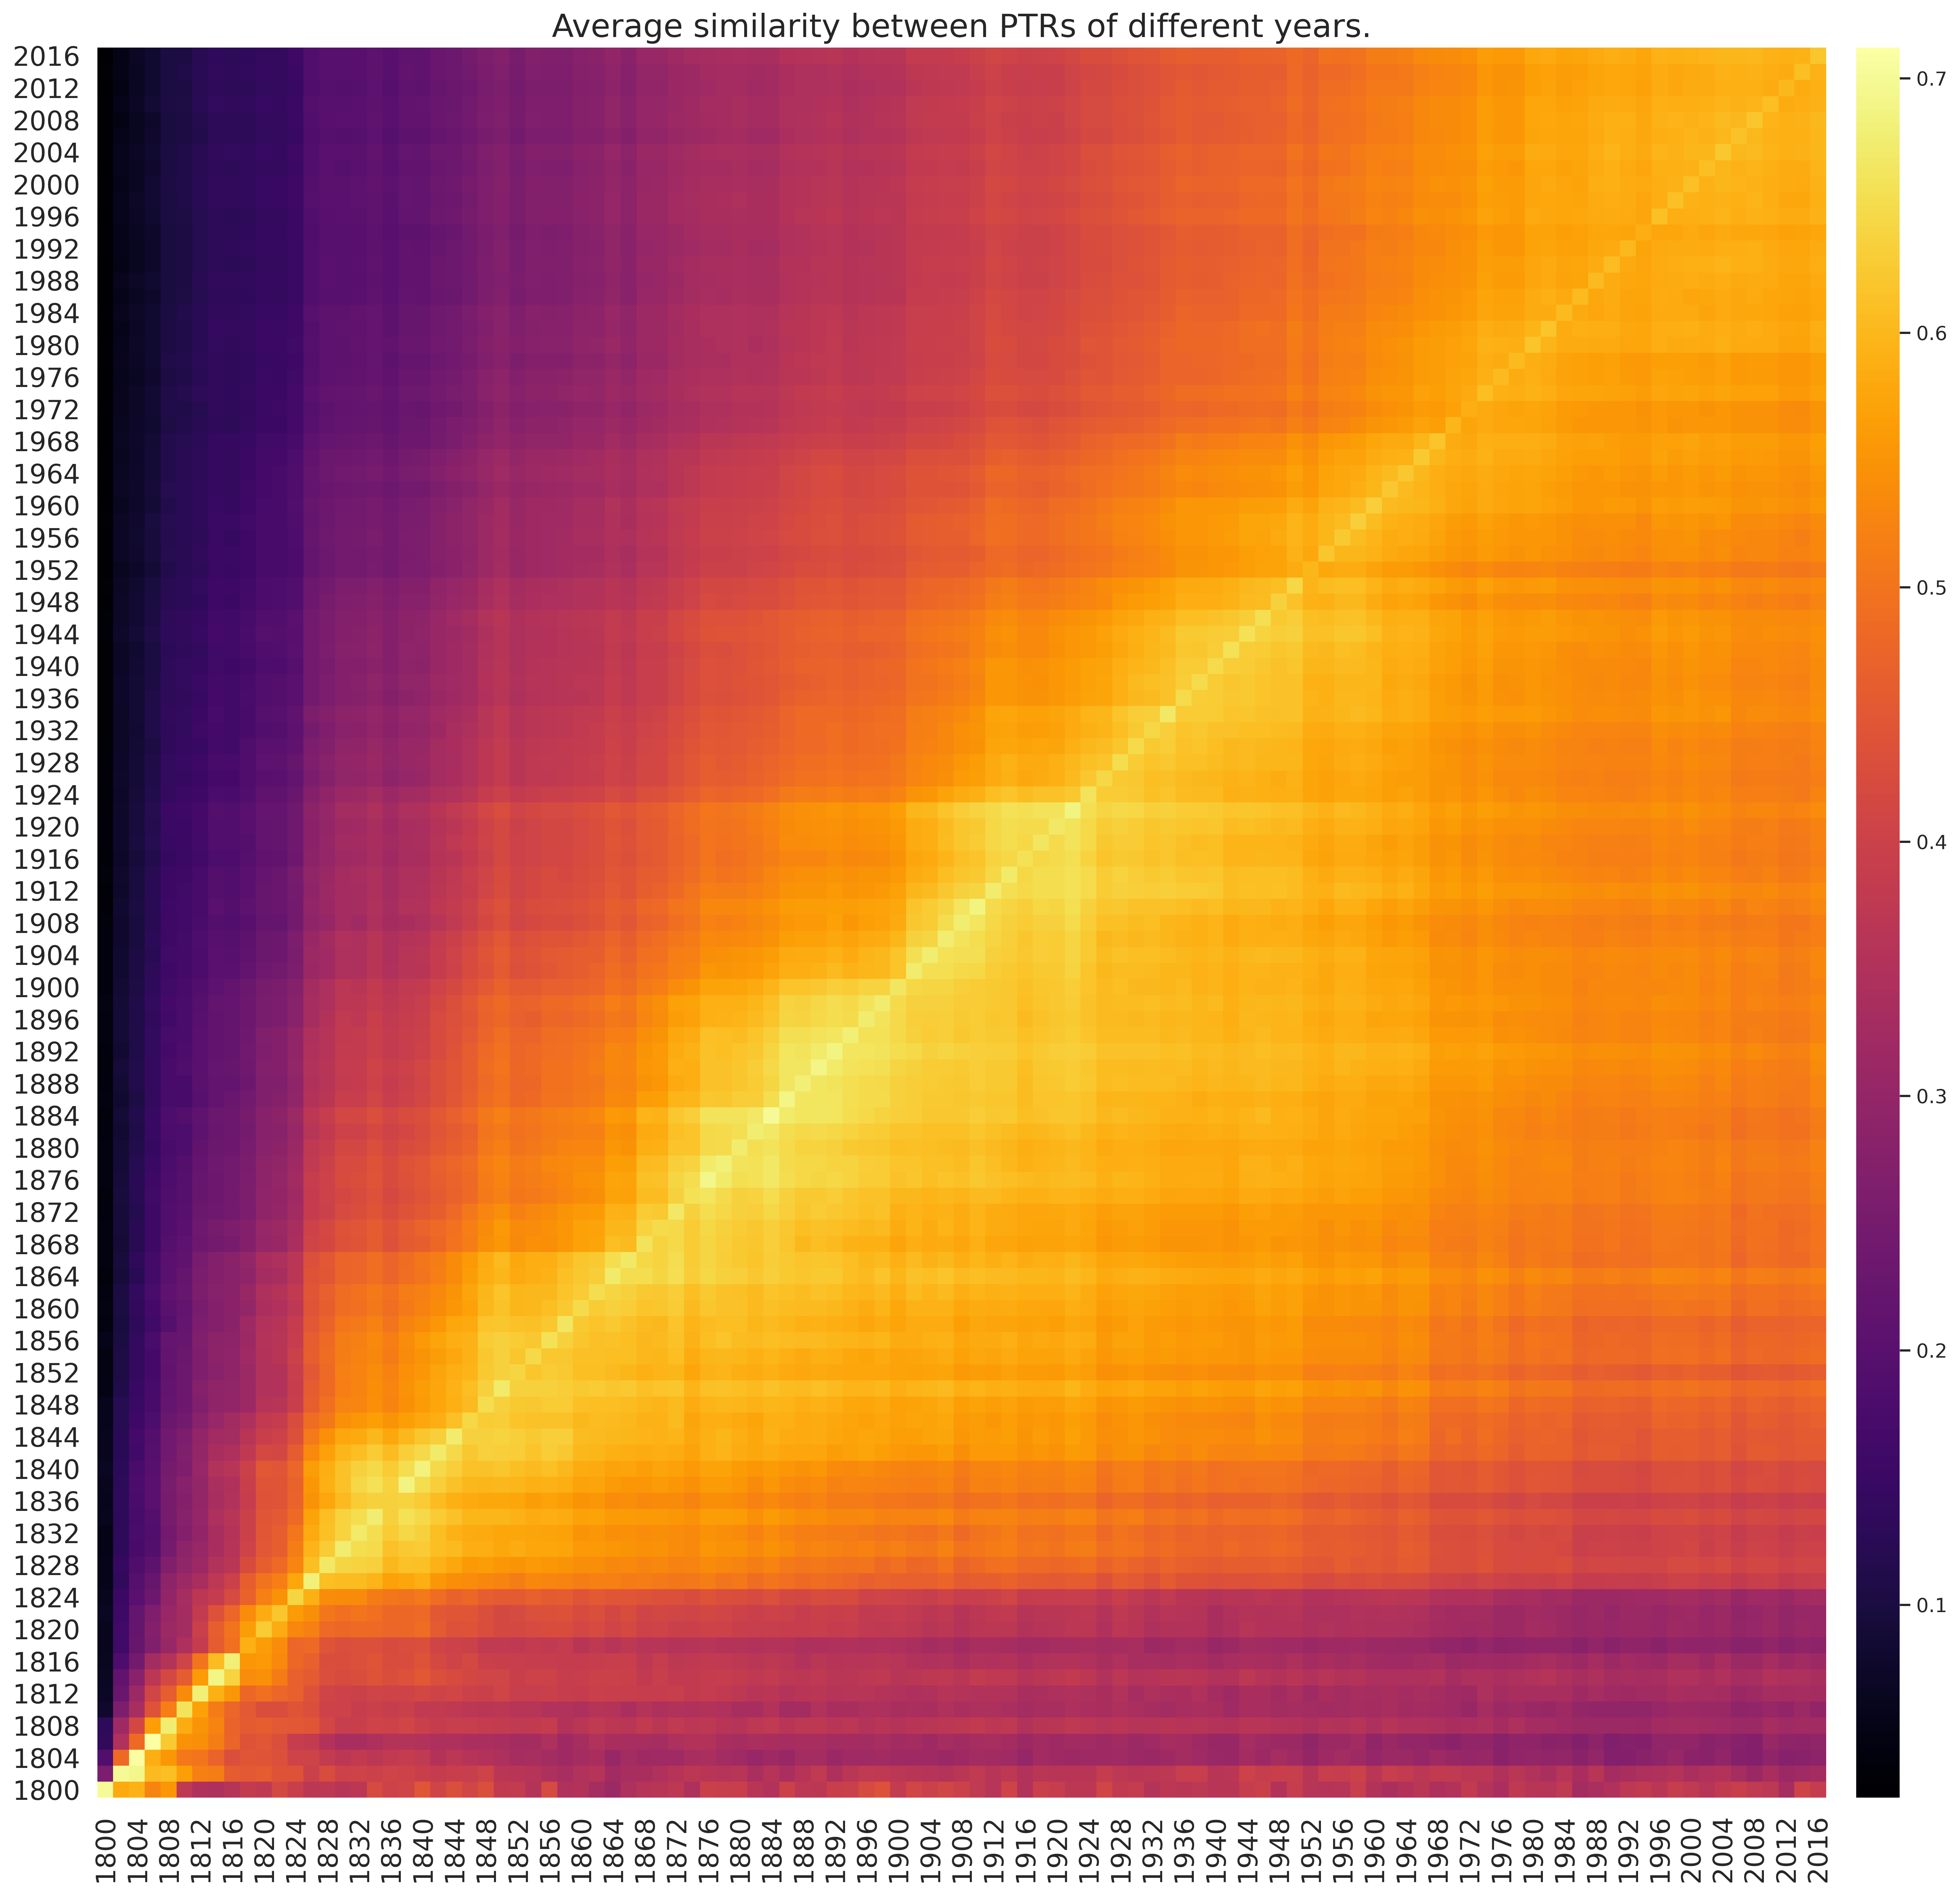
\includegraphics[width=18.0cm]{history_mat.png}
	\caption{Historical evolution of the Periodic System, extracted from 1D PTRs as a function of the evolving Chemical Space.}
	\label{fig:historicAnal}
\end{figure}

This plot is one of the most important results of this work, and represents one of the largest scale computational historical analyses performed to this date, both for the length of the period under consideration, and the amount of data effectively used each year, this last point being possible thanks to the size of the dataset itself, but also to the methodology used for its exploitation (Section \ref{sec:preprocessing}). 

As general conclusions from this plot it is observed that, very importantly, the PS indeed tends to converge to some stable form. This is reflected by the fact that, as the reader goes up observing the lower triangle, horizontal lines form with incresingly higher values, with no apparent significant variation on trends. That is what the bright triangle below the diagonal represents.
Second, the PS does indeed evolve, and some points in history can be found where somewhat abrupt changes occur. In particular, it is observed that before 1826, PSs would change rather randomly from year to year, as can be seen from the dark band to the bottom of the plot. In 1826, however, the picture changes rather abruptly, and the relationships found in this year are found to be preserved quite well along the history of the PS, particularly during the first ~150 years, but still being mantained up to 2016, the most recent year under study.\\
The conclusion here is that, given enough access to chemical data, processing capability and theoretical ideas, the chemical space had been explored well enough by 1826, to allow for a somewhat robust formulation of the periodic system; this is nearly 40 years before Mendeleev's and Meyer's independent publications of their systems.


\begin{figure}[h!]
  \centering
	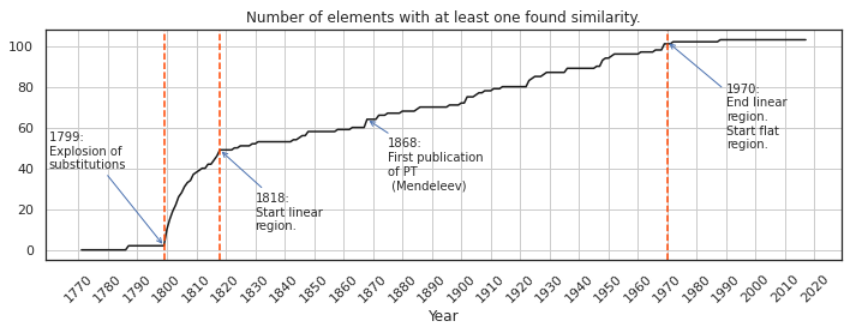
\includegraphics[width=18.0cm]{numberElems.png}
	\caption{Number of known elements as a function of time. Obtained from the database.}
	\label{fig:numElems_evol}
\end{figure}


Having found out that the PS tends to preserve a considerable amount of relationships between elements or groups of elements as it evolves with time, the question now is what, in particular, are these relationships that appear and are preserved throughout the history of the PS. In the same spirit of this work, the objective will now be to automatically extract groups of elements out of some given CS. Once such goal is achieved, history may be explored in a similar way, this time by exploring the evolution of each particular group and their relative importance in the structural stability of the PS, which may be assessed by means of the cost function devised for section \ref{sec:geneticAlgo}

\subsection{Automatic extraction of PS groups.}




%% HERE

\textbf{---------------------------------------------------------------}


Topics:

\begin{enumerate}
	\item [x] Introduce symmetric formulation of similarity matrix
	\item [x] Introduce optimization objective (cost function).
	\item [x] Briefly introduce opt method: Genetic algorithm, explain crossover + mutation scheme used.
	\item [x] Test the metrics on some known sequences
	\item [x] Introduce the problem of inevitable variability on results + non-direct-comparability of different resulting "optimal" sequences.
	\item [x] Introduce distance measurement between two different sequences
	\item [x] Show correlation between this distance and difference in their cost
	\item [x] With such distance measurement, you can now compare different results for the same year, BUT we can now compare two sequences optimized for different years as well, which results in some historical analysis.
	\item From the sequences we just got, can we automatically extract periodic table groups?
	\item Introduce the methods from computer vision that we're using for segmentation of re-sorted similarity matrix, and extraction of PT groups.
	
	
\end{enumerate}

The present work could take many different directions from this point. In particular, the approach developed here could be directed towards the optimization of a one-dimensional ordering of elements, such as that reported in \cite{Glawe_2016}, where a reformulation of the Pettifor's scale was done with a similar approach to that presented here, but using only a set of inorganic substances obtained from the \href{https://ucsd.libguides.com/crystallography/icsd}{ICSD}. Again, such work could highly benefit from the more general approach considered here with much more substances and relations, and the conclusions of such work could as easily be drawn.\\

%% OTHER HERE

Another direction is finding an optimal two-dimensional representation, that expresses a given order e.g. by atomic number), while expressing chemical similarity as well. In general, the investigation could be headed towards the optimization of a PS, given a dimensional constraint. As such, the question about the optimal dimensionality of a PS could be addressed, and all of this could be extended towards a historical analysis.\\

Equipped with def. \ref{def:def4}, this work will take the second approach mentioned: the optimization of a two-dimensional representation of the PS (PTR). For that matter, the expanded description provided by individual mHND$_i$s is dumped into a single number S, which will be the sum of a modified expression for all individual mHND$_i$s.

\begin{equation}
\label{eq:eq1}
	S = \sum_i mHND_i = \sum_i \frac{\sum_k M_{ik} (G_i - G_k)^2}{\sum_{k \neq i} M_{ik}}
\end{equation}

Where the absolute value is exchanged by the square operation. In that sense, the above equation represents a mean horizontal square distance, but for our purposes the focus will be on the quantity $S$ only. Such quantity will be our optimization objective. To begin, as we have an (in principle) analytical expression, gradients can be calculated as follows.

\begin{equation}
\frac{\partial S}{\partial G_j} = \sum_i \frac{ ( G_i - G_j ) N_{ij} }{\sum_k N_{ik} - N_{ii}}
\end{equation}

As \\
$$
\frac{\partial G_{k}}{\partial G_j} = 0, \forall k \neq j
$$

The advantage of our modified version of mHND (eq. \ref{eq:eq1}) is that the gradients of S contain explicit information about distances, while the gradient of absolute values would only contain information about the sign. With these quantities at hand, a variety of optimization techniques could be applied. \\


%% OLD:
\subsection{Evaluation of a PS: Horizontal Neighbouring Distance}


On the light of these results, a few questions arise:
\begin{itemize}
	\item How good does a selected PS express these patterns? 
	\item How would an optimal tabular representation of the PS look, on the light of such metrics?
	\item How does such representation evolve with time?
	\item How \textit{early} could we come up with a stable representation?
\end{itemize}



For the assessment of these, and many more questions, we formulate a \textit{fitness} measure, general for any tabular representation of the PS.



With the objective of comparing different periodic table representations of the PS (PTR), the aim of this chapter is to develop a measure for the adequateness of a particular PTR for describing the generalities of the relations between elements. \\

Although with well known exceptions, the general idea of a PTR is to encode both order and similarity between elements. In that sense, their construction requires an underlying, in principle sequential order (usually by atomic number), being \say{distorted} by similarity relations that are expressed in a second dimension through clasification of elements in a number of columns, which will be called groups. As the order relation is already fixed, our evaluation should be concerned with how well grouped are similar elements. Now, some degree of flexibility should be given to the proposition that similar elements be placed in exactly the same group; instead it may be proposed that similar elements should at least lie in neraby columns.\\

With such requirements in mind, the horizontal neighbouring distance (HND) is now proposed. Let us first understand what the calculation is about, and then a mathematical formula will be derived. First, let us assume elements X and Y are related by the similarity relationship (R,n). Assuming a PTR, such pair of elements have each an assigned group and as such, a \textit{horizontal distance} can be calculated between them neighbors. In order to include the information about every single binary relationship, the mean is calculated as the sum of all these distances, divided by the number of binary relationships.\\

Naturally, the distances between every pair of elements is fixed, for a fixed PTR. As such, the above described mean can just be computed as a mean of all the pairwise distances, weighted by the number of similarity relations found for each pair of elements. This statement is formalized through the following definitions.

\begin{definition}[Group vector]
\label{def:def3}
A group vector $G$ is a numeric array containing the group number of each element, in a particular PTR. The ith entry of $G$ corresponds to the group to which the ith element belongs in the given PTR. As such, $G$ is a functional of the PTR. $G=G[PTR]$.
\end{definition}

\begin{definition}[Mean Horizontal Neighbouring Distance]
\label{def:def4}
mHND is defined as the weighted average of all binary similarity relations among elements. Considering that matrix elements $M_{ij}$ (def. \ref{def:def1}) contain the weight for similarity relation between ith and jth elements, then mHND$_i$, for element i, is defined as follows.

	\begin{equation}
		mHND_{i} = \frac{\sum_k M_{ik} | G_i - G_k |}{\sum_{k \neq i} M_{ik}}
	\end{equation}
	
Where the sumation in the numerator can be written as such, as $G_i - G_i = 0$.
\end{definition}

By construction, a mHND$_i$ of 0 means that exactly all elements related to ith element by similarity relations, are in the same group in the given PTR as said element, reinforcing the vertical similarity idea, while a larger distance implies a departure from this rule. Figure \ref{fig:fig3} shows a plot of mHND for all elements, calculated using the long format of the periodic table and embedded in the same format.

%\begin{figure}[h!]
%  \centering
%	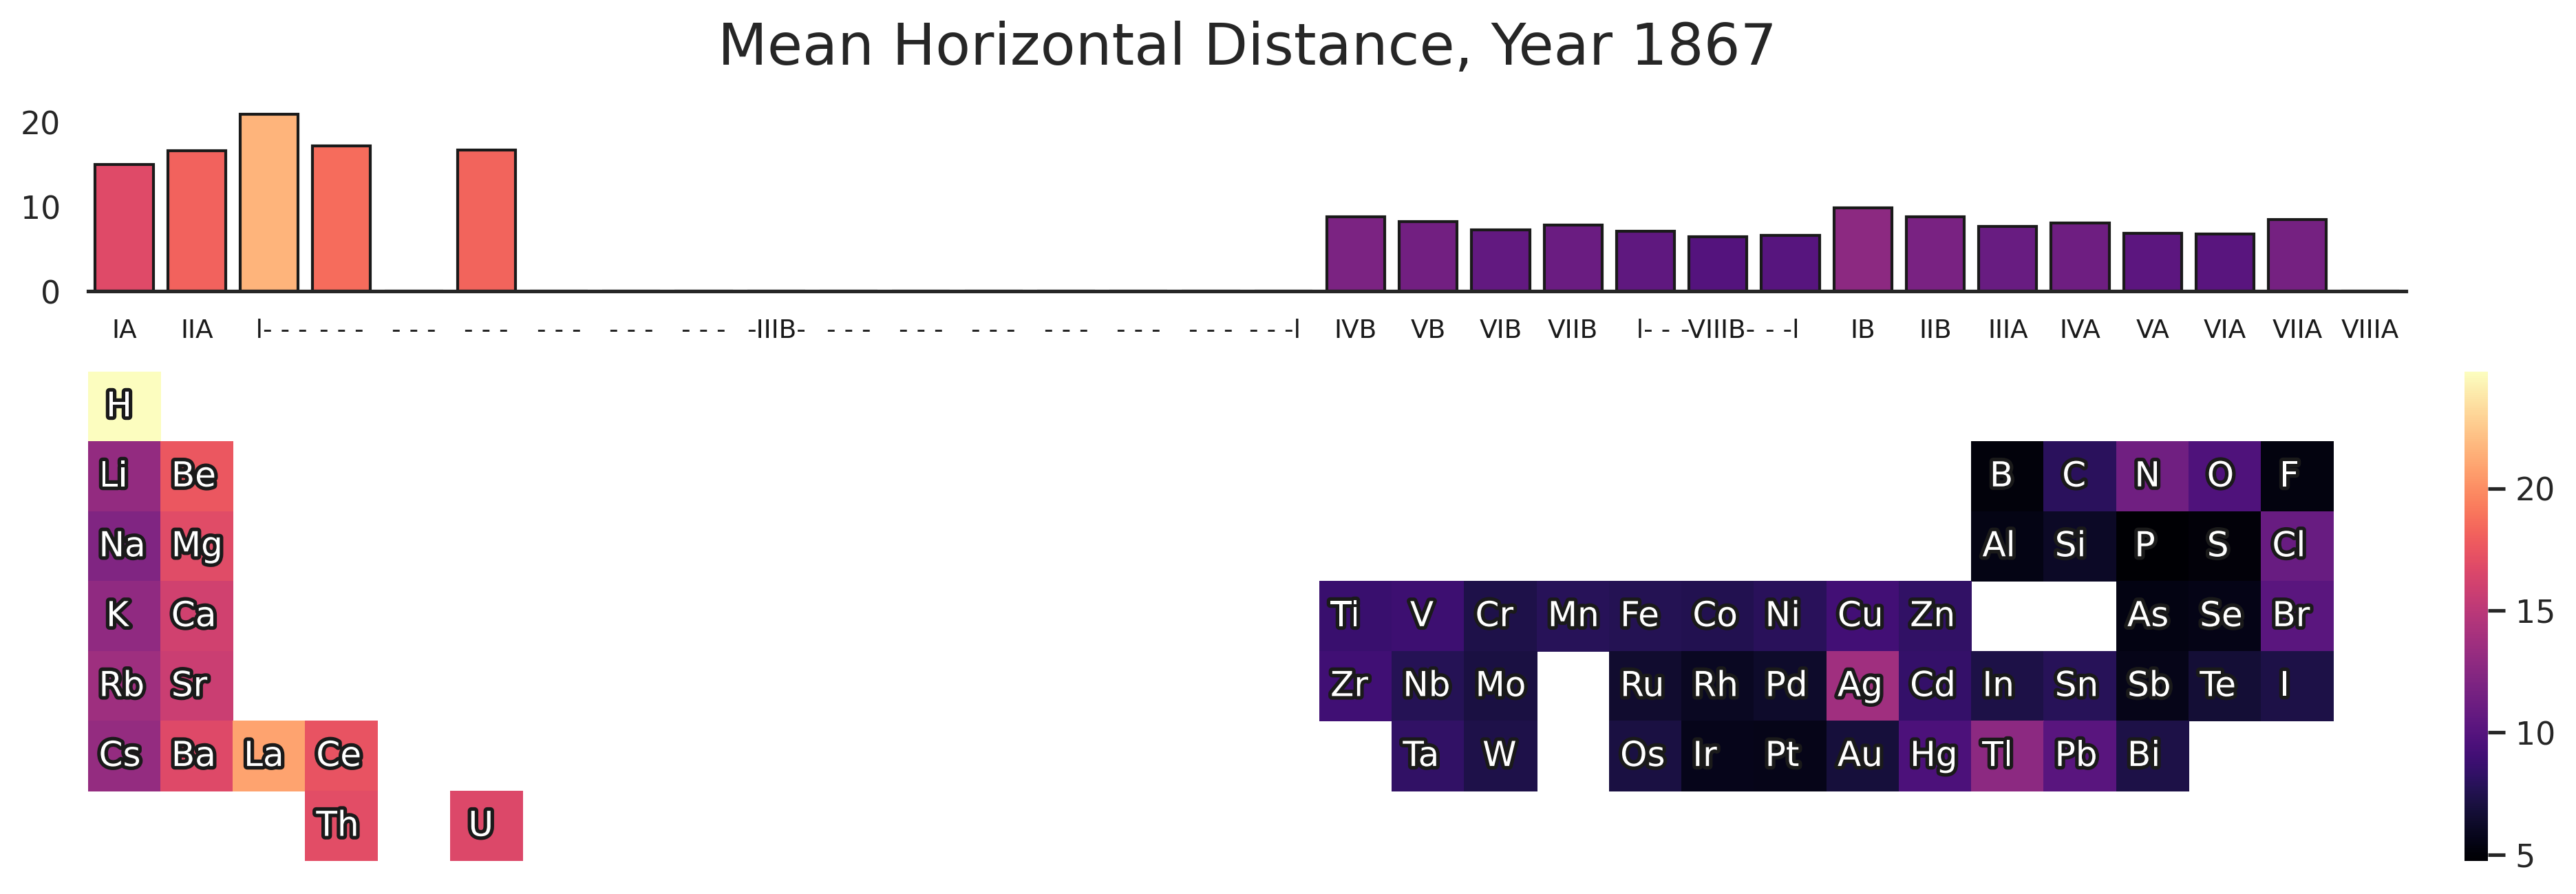
\includegraphics[width=18.0cm]{mHND_1868.png}
%	\caption{Mean horizontal neighboring distance (mHND) for the elements in the PS, year 1868.}
%	\label{fig:fig3}
%\end{figure}

Figure \ref{fig:fig3} clearly shows that, overall, the vertical similarities are not dominant the whole MPT and, furthermore, such patterns are observed more commonly to the right of such table. Groups 1 and 2 show surprisingly high mHNDs considering how chemically similar elements within these groups are expected to be (Na-K-Rb-Cs and Mg-Ca-Sr for instance). 

Given that mHND$_i$ is parametrically a function of the selected PTR, a new PTR may now be devised by optimization of this quantity, which would lead to one where mHND is minimized for every element, while preserving some given elemental ordering (be it atomic weight, Pettifor's scale, etc), which should naturally lead to a more expressive representation, and would allow a comparison between systems. Optimization and comparison between systems is a topic for the next section.\\



To facilitate the visualization of the first kind of representation (figures \ref{fig:fig3} and \ref{fig:fig4}) an interactive webpage is to be constructed, where the similarities are calculated for an user-chosen element and shown in the PS representation.
 
 

\renewcommand\refname{References}
\bibliography{bib}
\bibliographystyle{ieeetr}

\end{document}             % End of document.

